\documentclass{article}
\linespread{1.3}
\usepackage[margin=50pt]{geometry}
\usepackage{amsmath, amsthm, amssymb, amsthm, tikz, fancyhdr}
\pagestyle{fancy}
\renewcommand{\headrulewidth}{0pt}
\newcommand{\changefont}{\fontsize{15}{15}\selectfont}

\fancypagestyle{firstpageheader}
{
  \fancyhead[R]{\changefont Michael Huang \\ CFRM 415 \\ Homework 3}
}

\begin{document}

\thispagestyle{firstpageheader}

\section*{1.}

{\Large 

According to put-call parity, we know that \\
$C - P - S + PV(X) = 0$ \\
$C - P = S - PV(X)$ \\
$C = S - PV(X) + P$ \\
Since $P > 0$, we can see that \\
$C \geq S - PV(X)$ \\
as we aimed to show. \\ \\
% The time value of a call is more the than the time value of a corresponding put.
% Time value part is greater than just share price or loan?
This confirms that the time value is always positive for the European call option, as displayed by the difference between the lines.
% nonnegative?

\begin{figure}[h]
  \centering
  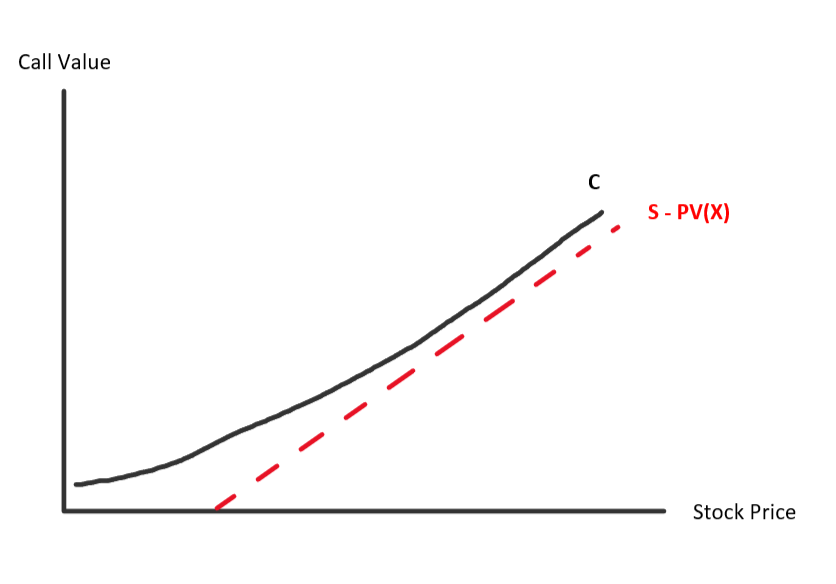
\includegraphics[width=120mm]{./1.png}
\end{figure}

\newpage

}

\section*{2.}
{\Large

\subsection*{(a)}

The trader believes that the stock price $S$ will go below $X$ at time $T$, the time at which they can then exercise the option. 
% Specifically, if the trader pays some premium $P$ on the option, then they would expect the stock price $S$ to go at least $P$ below $X$, or that $S$ will be at most $X - P$ at time $T$. 

\subsection*{(b)}

\begin{figure}[h]
  \centering
  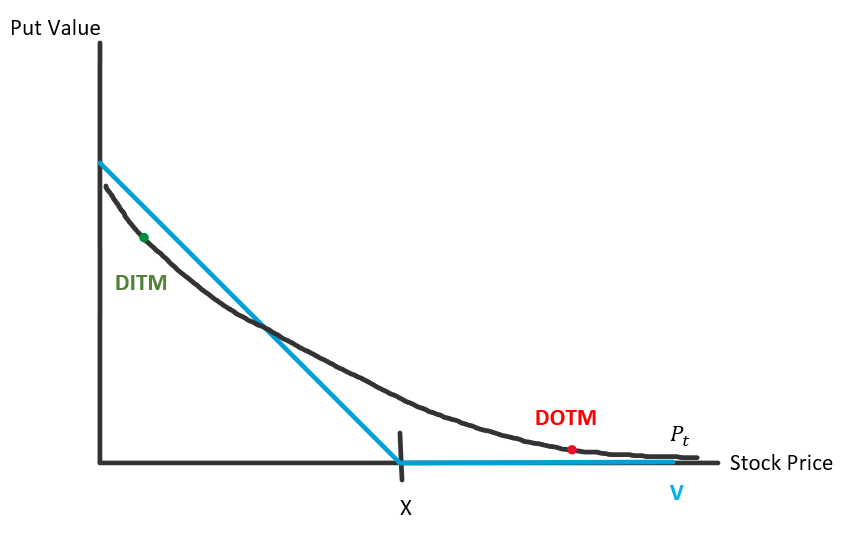
\includegraphics[width=120mm]{./2.png}
\end{figure}

\subsection*{(c)}

See part (b), labeled as $P_t$.

\subsection*{(d)}

See part (b), labeled as $DITM$. \\
The intrinsic value will be relatively high and positive. \\
The time value will be relatively low, and in our case according to the point we picked on the curve, even negative.

\subsection*{(e)}

See part (b), labeled as $DOTM$. \\ \\
The intrinsic value at this point is zero (we cannot exercise the put option for profit, so it is worthless). 
The time value will be higher in comparison with the time value at the point where we are deep in the money. 
% (greater chance of becoming more valuable, depends on t)
% could also be smol, depending on diff between option value at/before expiry

}

\section*{3.}
{\Large 

The European capped call option pays $H - X$ for $H > X$ when $S$ exceeds $H$, $S - X$ when $S$ exceeds $X$ but not $H$, and 0 otherwise. We aim to construct a portfolio of European options with identical payoff. \\ \\
We find that a possible portfolio of European options with identifical payoff consists of taking a long position on a European call with strike price $X$ and taking a short position on a European call with strike price $H$. We can see that this provides us with the same outcomes as the European capped call optin for the above 3 scenarios at expiry: \\ \\ 
$S > H$: Both options are exercised. The former has payoff of $S - X$, while the latter has payoff of $S - H$, which we negate since we are taking the short position, so our total payoff is now $S - X - (S - H) = S - X - S + H = -X + H = H - X$. \\
$X < S \leq H$: Only the former option is exercised, in which case we have a payoff of $S - X$, while the other payoff is 0 since it is now worthless. \\
$S \leq X$: Neither option can be exercised, so we are left with payoff of 0 from both for a total of 0. \\ \\
This shows that this portfolio as defined above will result in the same payoff as the European capped call option.

}

\end{document}